\documentclass[12pt,a5paper]{article}
\usepackage[a5paper,margin=6mm]{geometry}
\usepackage{graphicx}
\usepackage{amsmath,amsfonts,defns}
\usepackage{pgfplots}

\newcommand{\Bb}[1]{%
  \expandafter\def\csname#1#1\endcsname%
  {\ensuremath{\mathbb #1}}}
\Bb X\Bb T\Bb R\Bb I\Bb J

\usepackage{pdfcomment}
\newcommand{\ajr}[1]{%
  \pdfcomment[author=AJR,color={1 1 0},subject={#1}]{#1}}
\newcommand{\gaj}[1]{%
  \pdfcomment[author=GAJ,color={0 1 1},subject={#1}]{#1}}
\AtBeginDocument{\listofpdfcomments}

\title{Notes on the Diffusion Equation}

\begin{document}
\maketitle
\section{Introduction}
Consider an arbitrary solution $u:\XX\times \TT\mapsto \RR$ to the simple diffusion equation 
\begin{eqnarray}
	\D tu = \DD xu\,.
	\label{eq:diff}
\end{eqnarray}
A computationally feasible approach would be to 
first establish $|{\JJ}|$ discrete grid-points,
${\vec X}=[X_j]_{j\in\JJ}$, and thence
partition the spatial domain \XX\ into 
contiguous intervals \(\II_j:=(X_{j-1},X_j]\). 
The coarse dynamics at the grid-points are then summarised by
${\vec U}=[U_j]_{j\in\JJ}$, where $U_j(t)=u(X_j,t)$ for all $t\in \TT$, according to some temporal evolution
\begin{eqnarray}
	\dot{\vec U}(t) = {\vec g}({\vec U}(t))\,.
	\label{eq:temporal}
\end{eqnarray}
Consequently, a link from the coarse dynamics ${\vec U}$ back to the continuum dynamics $u$ might be provided
by choosing an appropriate spatial mapping of the form
\begin{eqnarray}
	u  := u(x,{\vec U}(t)).
	\label{eq:spatial}
\end{eqnarray}
Under this scheme, the linear diffusion equation~(\ref{eq:diff}) becomes
\begin{eqnarray}
	\D {\vec U}{u}\cdot{\vec g} = \DD x{u}\,.
	\label{eq:diff2}
\end{eqnarray}
Observe that the evolution of $u$ now has nonlinear interactions with ${\vec U}$.

\section{Centre Manifold Approximation}\label{sec:centre-man}
The original diffusion equation~(\ref{eq:diff}) admits 
eigensolutions of the form
\begin{eqnarray}
	u(x,t)  = e^{\lambda t+ikx}\,,
\label{eq:raw-eigmode}
\end{eqnarray}
which are physically realisable for real eigenvalues $\lambda=-k^2\le 0$ for 
corresponding eigenmode wavenumbers $\pm k$. 
As a consequence, the transient solutions corresponding
to $\lambda<0$ decay rapidly to the centre manifold corresponding to $\lambda=0$. 

This centre manifold can be found in practice by iteratively refining approximations to $u$. In particular, consider a series expansion of the form
\begin{eqnarray}
	u  & \sim & \hat{u}_0+\gamma\hat{u}_1+\gamma^2\hat{u}_2+\cdots\,,
\label{eq:u:series}
\end{eqnarray}
for some parameter $0\le\gamma\le 1$.
Now, the constant eigensolution for $\lambda=0$ implies a slow evolution for the coarse dynamics given by 
equation~(\ref{eq:temporal}), which therefore admits a series expansion of the form
\begin{eqnarray}
	\dot{{\vec U}} & \sim & \gamma {\vec g}_1+\gamma^2 {\vec g}_2+\cdots\,.
\label{eq:Udot:series}
\end{eqnarray}
Hence, equation~(\ref{eq:diff2}) may be decomposed at each order 
$\ell$ of the parameter $\gamma$, giving
\begin{eqnarray}
   \DD {x}{\hat{u}_0} & = & 0\,, \label{eq:pert1}
\\
  \DD {x}{\hat{u}_\ell} & = & \sum_{m=0}^{\ell-1}\D {\vec U}{\hat{u}_m}\cdot{\vec g}_{\ell-m}\,,
\hspace*{5mm}\mbox{for }\ell=1,2,\ldots\,.
\label{eq:pert_ell}
\end{eqnarray}


\section{Leading Approximation}
The leading equation~(\ref{eq:pert1}) admits any spatially piecewise linear function as a solution. 
Hence, in keeping
with the discretisation imposed by the coarse dynamics, 
consider the linear approximation
\begin{eqnarray}
   \hat{u}_0 = \sum_{j\in\JJ}\chi_j(\xi_j U_j+(1-\xi_j)U_{j-1})\,,
\label{eq:uhat0}
\end{eqnarray}
with indicator $\chi_j(x)=1$ (or 0) for $x\in\II_j$ (or $x\not\in\II_j$), and interpolator
$\xi_j(x)=\frac{x-X_{j-1}}{X_j-X_{j-1}}$.
This particular approximation is chosen to be continuous across the boundaries of each interval $\II_j$. 
In general, it suffices 
to impose a continuity condition at the right-hand end of each $\II_j$, namely:
\begin{eqnarray}
   [u]_j := \lim_{\epsilon\rightarrow 0^{+}} u(X_j+\epsilon,t)-u(X_j-\epsilon,t)= 0\,.
\label{eq:cont-cond}
\end{eqnarray}
Unfortunately, this linear approximation is not smooth at the interval boundaries. 
For convenience, consider regular grid spacings of size 
$X_j-X_{j-1}=H$. Then, denoting $\D xu$ as $u'$, observe that
\begin{eqnarray}
   [\hat{u}'_0]_j = \frac{1}{H}(U_{j+1}+U_{j-1}-2U_j)~=~\frac{1}{H}\left.\delta^{2}\hat{u}_0\right|_{X_j}\,,
\end{eqnarray}
for the centred difference $\delta u(x,t):= u(x+\frac{H}{2},t)-u(x-\frac{H}{2},t)$\,.
However, this non-smoothness may be corrected at higher order by imposing a further internal boundary condition, namely
\begin{eqnarray}
   [u']_j = \frac{1-\gamma}{H}\left.\delta^{2}u\right|_{X_j}\,.
\label{eq:smooth-cond}
\end{eqnarray}
Consequently, smooth approximations are found in the limit as $\gamma\rightarrow 1$.

\section{Linear Eigenmode Analysis}\label{sec:eig:modes}
Consider a single eigenmode of the form~(\ref{eq:raw-eigmode}) for some fixed, non-dimensionalised 
wavenumber $\kappa=kH>0$. 
Thus, allowing for the partitioning of \XX, let
\begin{eqnarray}
u & \sim & \sum_{j\in\JJ} \chi_j a_j e^{i\kappa\xi_j} + \text{c.c.}\,,
\end{eqnarray}
for arbitrary, time--varying, complex coefficients $a_j=A_j+iB_j$. 
We now seek the `spatial' evolution from interval to interval for the given wavenumber.
The continuity condition~(\ref{eq:cont-cond}) implies that
\begin{eqnarray}
a_{j+1} - a_j e^{i\kappa\xi_j} + \text{c.c.} = 0\,.
\end{eqnarray}
Similarly, the smoothness condition~(\ref{eq:smooth-cond}) implies that 
\begin{eqnarray}
ik a_{j+1} -ik a_j e^{i\kappa} + \text{c.c.} =  
\frac{1-\gamma}{H}\left(
a_{j+1} e^{i\kappa} + a_j - 2 a_j e^{i\kappa}
\right)
+ \text{c.c.}\,,
\end{eqnarray}
where continuity has also been invoked at the left-hand of the $j$th interval.
In coefficient form, the update from the $j$th to $(j+1)$th segment is
\begin{eqnarray}
\left[\begin{array}{cc}
1 & 0\\
fc & 1-fs\\
\end{array}\right]
\left[\begin{array}{c}
A_{j+1}\\
B_{j+1}\\
\end{array}\right]
=
\left[\begin{array}{cc}
c & -s\\
s+f(2c-1) & c-2fs\\
\end{array}\right]
\left[\begin{array}{c}
A_{j}\\
B_{j}\\
\end{array}\right]\,,
\end{eqnarray}
where $c+is:=e^{i\kappa}$ and $f:=\frac{1-\gamma}{\kappa}$.
Now, letting $a_{j+1}=\mu a_j$, the characteristic equation for 
the growth factor $\mu$ is
\begin{eqnarray}
(1-fs)\left[\mu^2-2\frac{c-fs}{1-fs}\mu+1\right] = 0\,,
\end{eqnarray}
with roots given by
\begin{eqnarray}
\mu & = & \beta\pm\sqrt{\beta^2-1}
\hspace*{5mm}\mbox{for } 
\beta~=~\frac{c-fs}{1-fs}\,.
\end{eqnarray}
Observe that $\beta\le 1$ since $c=\cos\kappa\le 1$ and 
$1-fs=1-(1-\gamma)\frac{\sin\kappa}{\kappa}\ge 0$.
Thus, for $|\beta|<1$, the factors are complex with magnitude 
$|\mu|=1$,
indicating marginally stable evolution of $a_j$. 
This includes the limiting case of $\gamma=1$ ($f=0$), for which
$\mu=c\pm is=e^{\pm i\kappa}$.
Likewise, $\mu=\pm 1$ for $\beta=\pm 1$, corresponding to $\kappa=n\pi$, $n=0,1,2,\ldots$.
Finally, for small regions near each $\kappa=(2n+1)\pi$, 
it is found that $\beta<-1$, resulting in two real factors,
$\mu<-1$ and $-1<\mu<0$, indicating unstable (saddle) evolution.
More precisely, these unstable regions occur when
\begin{eqnarray}
%c-fs < -(1-fs) & \Rightarrow & 1+c < 2fs 
%\frac{kH}{1-\gamma}\cos^2\frac{kH}{2} < 2\sin\frac{kH}{2}\cos\frac{kH}{2}\,.
\frac{\kappa}{2} <(1-\gamma)\tan\frac{\kappa}{2}\,, && \kappa\ne n\pi\,.
\label{eq:leaforbid}
\end{eqnarray}
Thus, at equilibrium ($\gamma=0$) there is an initial forbidden gap $\kappa\in(0,\pi)$ adjacent to the centre manifold
wavenumber $\kappa=0$ (see Figure~\ref{fig:leaspec}), indicating that transient solutions decay to the centre manifold at a rate of at least
$\lambda=-\frac{\kappa^2}{H^2}=-\frac{\pi^2}{H^2}$. It is this gap that provides robustness to nonlinear perturbations
of the system about the equilibrium.

\begin{figure}[hbt]
\centering
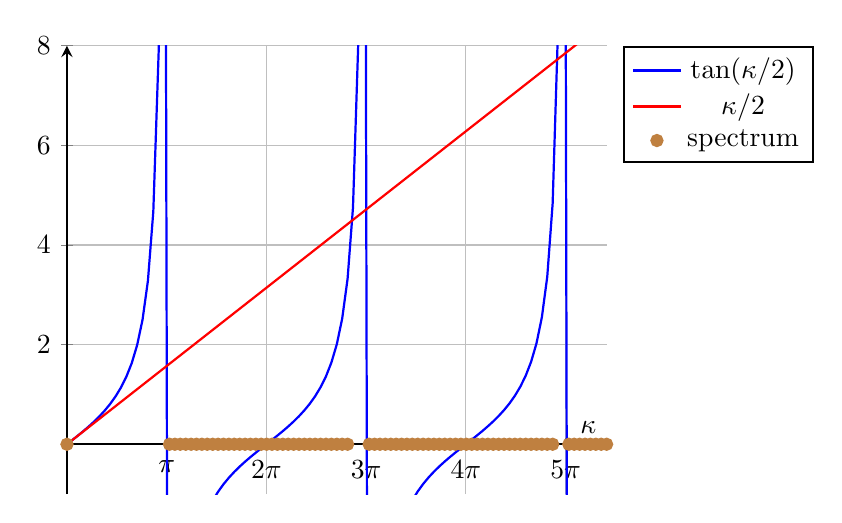
\begin{tikzpicture}
\begin{axis}[ xlabel={$\kappa$}
  ,axis x line=middle,axis y line=middle
  ,thick,grid,samples=101
  ,ymin=-1,ymax=8 ,domain=0:17
  ,xtick={3.1416,6.2832,9.4248,12.5664,15.7080}
  ,xticklabels={$\pi$,$2\pi$,$3\pi$,$4\pi$,$5\pi$}
  ,legend pos=outer north east
  ] 
\addplot [blue,no marks] {tan(deg(x)/2)}; 
\addlegendentry{$\tan(\kappa/2)$};
\addplot [red,no marks,samples=2] {x/2}; 
\addlegendentry{$\kappa/2$};
\addplot [brown,only marks,mark=*] {0-99*(x/2<tan(deg(x)/2))};
\addlegendentry{spectrum};
\end{axis}
\end{tikzpicture}
\caption{The equilibrium spectrum determined by the forbidding condition~\eqref{eq:leaforbid}.}
\label{fig:leaspec}
\end{figure}


\section{Linear Dual Space}
Suppose the domain \XX has been discretised to have outer boundaries $X_{\underline{J}}$ and $X_{\bar{J}}$ for indices
$\underline{J}=\inf{\JJ}$ and $\bar{J}=\sup{\JJ}$. Assume for convenience that $|\JJ|> 2$.
Then an appropriate inner product for spatially square-integrable fields $u$ and $v$ is given by
\begin{eqnarray}
\langle u,v\rangle = \int_{X_{\underline{J}}}^{X_{\bar{J}}}uv\;dx
= \sum_{j=\underline{J}+1}^{\bar{J}}\int_{\II_j}uv\;dx\,.
\end{eqnarray}
It can then be shown, for twice-differentiable fields, that
\begin{eqnarray}
\langle u'',v\rangle =
\langle u,v''\rangle + R\,,
\end{eqnarray}
with residual 
\begin{eqnarray}
R &= & \sum_{j=\underline{J}+1}^{\bar{J}}[r]_{X_{j-1}}^{X_j}
= r_{\bar{J}}-r_{\underline{J}}-\sum_{j=\underline{J}+1}^{\bar{J}-1}[r]_j\,,
\end{eqnarray}
for $r=u'v-v'u$.
Now, assuming that both $u$ and $v$ obey conditions~(\ref{eq:cont-cond}) and~(\ref{eq:smooth-cond}), 
the residual jump at $X_j$ becomes
\begin{eqnarray}
[r]_j & = & [u']_j V_j-[v']_j U_j
\nonumber\\
& = & \frac{1-\gamma}{H}\left[
(U_{j+1}+U_{j-1})V_j-(V_{j+1}+V_{j-1})U_j
\right]\,.
\end{eqnarray}
Observe that terms from adjacent intervals $\II_{j-1}$ and $\II_{j+1}$ will cancel terms from $\II_j$, leaving
only contributions from the outermost boundary intervals $\II_{\underline{J}+1}$ and $\II_{\bar{J}}$; consequently:
\begin{eqnarray}
R & = & 
u'_{\bar{J}}V_{\bar{J}}-v'_{\bar{J}}U_{\bar{J}}
-u'_{\underline{J}}V_{\underline{J}}+v'_{\underline{J}}U_{\underline{J}}
\nonumber\\ &&
{}-\frac{1-\gamma}{H}\left[
U_{\bar{J}}V_{\bar{J}-1}-V_{\bar{J}}U_{\bar{J}-1}
+U_{\underline{J}}V_{\underline{J}+1}-V_{\underline{J}}U_{\underline{J}+1}
\right]\,.
\end{eqnarray}
On a finite domain, there are three main outer boundary conditions that lead to a zero residual:
\begin{description}
\item[periodic] Having period $\bar{J}-\underline{J}$ corresponds to \(U_{\bar{J}}=U_{\underline{J}}\). Furthermore, by joining
the domain cylindrically at $X_{\underline{J}}$ and $X_{\bar{J}}$,  it can be shown that
\begin{eqnarray}
u'_{\underline{J}}-u'_{\bar{J}} = [u']_{\bar{J}} = \frac{1-\gamma}{H}(U_{\underline{J}+1}+U_{\bar{J}-1}-2U_{\bar{J}})\,,
\end{eqnarray}
using condition~\eqref{eq:smooth-cond}. Hence, $R=0$ if correspondingly $v$ is periodic with period $\bar{J}-\underline{J}$.
\item[Dirichlet] Setting \(u=0\) at the boundaries corresponds to \(U_{\underline{J}}=U_{\bar{J}}=0\), 
giving $R=0$ if correspondingly \(v=0\) on the boundaries.
\item[Neumann] Requiring \(u'=0\) on the boundaries  (for $\gamma=1$) corresponds to 
\begin{eqnarray}
u'_{\underline{J}}=\frac{1-\gamma}{H}(U_{\underline{J}+1}-U_{\underline{J}})\,,
&&
u'_{\bar{J}}=\frac{1-\gamma}{H}(U_{\bar{J}}-U_{\bar{J}-1})\,,
\end{eqnarray}
giving $R=0$ if correspondingly \(v'=0\) on the boundaries.
\end{description}
Under any of the above three conditions, observe that $\langle{\cal L}u,v\rangle =\langle u,{\cal L}v\rangle$
for ${\cal L}=\DD {x}{}$, and hence ${\cal L}$ is self-adjoint.
Furthermore, we are free to choose any dual $v$, e.g.\ to satisfy ${\cal L}v=0$ for conenience.
In particular, we may specifically target the $j$-th interval for $u$, for each $j\in\JJ$,  with $v=\hat{v}_0^{[j]}$, where
\begin{eqnarray}
\hat{v}_0^{[j]} = \chi_j\xi_j + \chi_{j+1}(1-\xi_{j+1})\,,
\label{eq:vhat0}
\end{eqnarray}
which satisfies conditions~\eqref{eq:cont-cond} and~\eqref{eq:smooth-cond} for $\gamma=0$.
It can then be shown in general that
\begin{eqnarray}
\langle u'', \hat{v}_0^{[j]}\rangle = -[u']_j+\frac{1}{H}\left.\delta^2 u\right|_{X_j}\,,
\label{eq:udd:vhat0}
\end{eqnarray}
for any continuous, twice-differentiable $u$.

\section{First-order Approximation}\label{sec:first-order}
Substituting the leading approximation~(\ref{eq:uhat0}) into the
nonlinear diffusion equation~(\ref{eq:pert_ell}) for $\ell=1$ results in
the first-order equation
\begin{eqnarray}
\hat{u}''_1 = \sum_{j\in\JJ}\chi_j(\xi_j g_{1,j}+(1-\xi_j)g_{1,j-1})\,.
\label{eq:uhat:1:dd}
\end{eqnarray}
Spatial integration then gives
\begin{eqnarray}
\hat{u}'_1 & = & \frac{H}{2}\sum_{j\in\JJ}\chi_j(\xi^2_j g_{1,j}
-(1-\xi_j)^2g_{1,j-1}+c_{1,j})\,,
\label{eq:udhat1}
\\
\hat{u}_1 & = & \frac{H^2}{6}\sum_{j\in\JJ}\chi_j(\xi^3_j g_{1,j}
+(1-\xi_j)^3g_{1,j-1}+3\xi_{j}c_{1,j}+d_{1,j})\,.
\label{eq:uhat1}
\end{eqnarray}
Recall from the chosen  spatial discretisation that $u|_{X_j}=U_{j}$ at each grid-point.
Observe this is already satified by $\hat{u}_0$ from equation~(\ref{eq:uhat0}), implying
from expansion~(\ref{eq:u:series}) that
\begin{eqnarray}
\left.\hat{u}_\ell\right|_{X_j}=0 && \mbox{for }\ell=1,2,\ldots\,.
\label{eq:u_ell_fixed}
\end{eqnarray}
Thus $[\hat{u}_\ell]_j=0$, satisfying the continuity 
condition~(\ref{eq:cont-cond}), and $\delta^2\hat{u}_\ell|_{X_j}=0$.
Now, evaluating equation~(\ref{eq:uhat1}) at $\xi_j=0$ gives $d_{1,j}=-g_{1,j-1}$,
and at $\xi_j=1$ gives $3c_{1,j}=-(g_{1,j}-g_{1,j-1})$.
Thus,  from equation~(\ref{eq:udhat1}), observe that
\begin{eqnarray}
[\hat{u}'_1]_j = -H\left(1+\frac{1}{6}\delta^2\right)g_{1,j}\,.
\end{eqnarray}
However, the smoothness condition~(\ref{eq:smooth-cond}) gives
\begin{eqnarray}
   [\hat{u}'_1]_j = 
\frac{1}{H}\left.\delta^{2}\hat{u}_1\right|_{X_j}
-\frac{1}{H}\left.\delta^{2}\hat{u}_0\right|_{X_j}
= -\frac{1}{H}\delta^{2}U_j\,,
\label{eq:udhat1-jump}
\end{eqnarray}
and hence
\begin{eqnarray}
\left(1+\frac{1}{6}\delta^2\right)g_{1,j} = \frac{1}{H^2}\delta^2U_j\,.
\label{eq:g1}
\end{eqnarray}
This solution can also be otained more directly via the dual space by computing $\langle\hat{u}''_1,\hat{v}_0^{[j]}\rangle$ from
equations~\eqref{eq:vhat0} and~\eqref{eq:uhat:1:dd}, and using results~\eqref{eq:udd:vhat0} and~\eqref{eq:udhat1-jump}.

Consequently, as a first approximation, the coarse dynamics evolve according to
\begin{eqnarray}
	\dot{\vec U} = \frac{\gamma}{H^2}S\delta^2\vec U + {\cal O}(\gamma^2)\,,
\end{eqnarray}
from equations~\eqref{eq:temporal} and~\eqref{eq:Udot:series},
where, for convenience, we let $S=(1+\frac{1}{6}\delta^2)^{-1}$.
Now, recall from Section~\ref{sec:centre-man} that the eigensolution $u=e^{\lambda t+ikx}$ %%~\eqref{eq:raw-eigmode} 
to the diffusion equation~\eqref{eq:diff} has the exact spectrum $\lambda=-k^2$.
It can further be shown that this eigensolution  satisfies the relation 
$\delta^2u=-2(1-\cos kH)u$. Hence, the spectrum of the first-order approximation with $\gamma=1$ is
given by
\begin{eqnarray}
\lambda = -\frac{6(1-\cos kH)}{H^2(2+\cos kH)} \sim -k^2-\frac{1}{12}H^2k^4+{\cal O}(H^4k^6)\,,
\label{eq:spec:1st}
\end{eqnarray}
which reveals an error of size ${\cal O}(H^2k^4)$ in comparison to the exact spectrum.
The behaviour of this approximate spectrum is shown in Figure~\ref{fig:spec:first-order}.
%% \cos kH \sim 1-k^2H^2/2+k^4H^4/24-O(k^6H^6).
%% -2(1-\cos kH) \sim -k^2H^2+k^4H^4/12-...
%% 1/(2+\cos kH) \sim 1/3(1-k^2H^2/6+...) = (1/3)*(1+k^2H^2/6-...)
%% -6(1-\cos kH)/(2+\cos kH) \sim (-k^2H^2+k^4H^4/12+...)*(1+k^2H^2/6+...)  = -k^2H^2-k^4H^4/6+k^2H^2/12+...
%%  = -k^2H^2-k^4H^4/12+...
\begin{figure}[hbt]
\centering
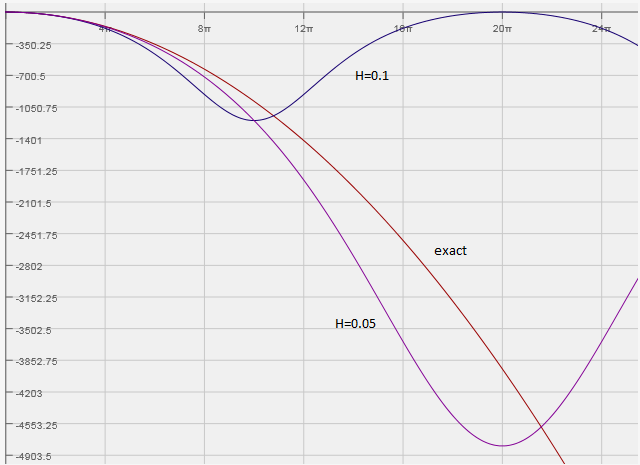
\includegraphics[width=0.8\textwidth]{figures/first-order-spectrum.png}
\caption{The exact spectrum ($\lambda$ versus $k$) of the linear diffusion equation, compared to a first-order approximation with $H=0.1$ and $H=0.05$, respectively, for $\gamma=1$.}
\label{fig:spec:first-order}
\end{figure}


\section{Second-order Approximation}
For convenience, consider the shift operator $\sigma u(x,t) := u(x+H,t)$;
 whence $\delta:=\sigma^{\frac{1}{2}}-\sigma^{-\frac{1}{2}}$.
Then, from equation~\eqref{eq:pert_ell} for $\ell=2$, we obtain
\begin{eqnarray}
  \hat{u}''_2 & = & \D{\vec U}{\hat{u}_0}\cdot{\vec g}_{2}+\D{\vec U}{\hat{u}_1}\cdot{\vec g}_{1}
\nonumber\\
& = & \sum_{j\in\JJ}\chi_j\left\{\xi_j+(1-\xi_j)\sigma^{-1}\right\}g_{2,j}
\nonumber\\
&& {}+\frac{1}{6}\sum_{j\in\JJ}\chi_j\xi_j(1-\xi_j)\left\{
(\xi_j-2)\sigma^{-1}-(\xi_j+1)
\right\}S\delta^2g_{1,j}\,,
\label{eq:uhat2:dd}
\end{eqnarray}
using equations~\eqref{eq:uhat0} , \eqref{eq:uhat1}, and~\eqref{eq:g1}.
Next, observe 
from equations~\eqref{eq:udd:vhat0}, \eqref{eq:smooth-cond} and \eqref{eq:u_ell_fixed} that
\begin{eqnarray}
\langle\hat{u}''_\ell,\hat{v}_0^{[j]}\rangle=0 && \mbox{for }\ell=2,3,\ldots\,.
\end{eqnarray}
Alternatively, it can be shown by direct integration and simplification that
\begin{eqnarray}
\langle\hat{u}''_2,\hat{v}_0^{[j]}\rangle = HS^{-1}g_{2,j}-\frac{H}{6}\left(\frac{7}{60}\delta^2+\frac{1}{2}\right)S\delta^2g_{1,j}\,,
\end{eqnarray}
from equations~\eqref{eq:vhat0} and~\eqref{eq:uhat2:dd}.
Hence, as a second approximation, the coarse dynamics evolve according to
\begin{eqnarray}
	\dot{\vec U} = \frac{\gamma}{H^2}S\delta^2\vec U 
+ \frac{\gamma^2}{60H^2}(7-2S)S^2\delta^4\vec U
+ {\cal O}(\gamma^3)\,,
\end{eqnarray}
using the fact that $S\delta^2=6(1-S)$.
%%on div; off allfac; factor h,k,gamma;
%%let k^8 => 0;
%%c:=1-k^2H^2/2+k^4*H^4/24-k^6*h^6/720;
%%Dsq:=-2*(1-c); Si:=1+Dsq/6;
%%S:=1-(Si-1)+(Si-1)^2-(Si-1)^3;
%%lam:=gamma*S*Dsq/H^2+gamma^2*(7-2*S)*S^2*Dsq^2/(60*H^2);
%%lam -> -k^2+H^4*k^6/180+O(H^6k^8)
Thus, following Section~\ref{sec:first-order}, the approximate spectrum for $\gamma=1$ is now
\begin{eqnarray}
\lambda = -\frac{1}{5H^2}\frac{96+27c-72c^2-51c^3}{8+12c+6c^2+c^3}
\sim -k^2-\frac{1}{180}H^4k^6+{\cal O}(H^6k^8)\,,
\end{eqnarray}
where, as previously in Section~\ref{sec:eig:modes}, $c:=\cos kH$.
Observe that the $O(H^2k^4)$ error term from the first-order approximation~\eqref{eq:spec:1st} has now been
completely eliminated by the second-order correction, in favour of an $O(H^4k^6)$ error.

The behaviour of this corrected, approximate spectrum is shown in Figure~\ref{fig:spec:2nd-order}.
Observe that the approximation becomes untenable from the first turning point, at which $k\approx\frac{\pi}{H}$.
%% \cos kH \sim 1-k^2H^2/2+k^4H^4/24-O(k^6H^6).
%% -2(1-\cos kH) \sim -k^2H^2+k^4H^4/12-...
%% 1/(2+\cos kH) \sim 1/3(1-k^2H^2/6+...) = (1/3)*(1+k^2H^2/6-...)
%% -6(1-\cos kH)/(2+\cos kH) \sim (-k^2H^2+k^4H^4/12+...)*(1+k^2H^2/6+...)  = -k^2H^2-k^4H^4/6+k^2H^2/12+...
%%  = -k^2H^2-k^4H^4/12+...
\begin{figure}[hbt]
\centering
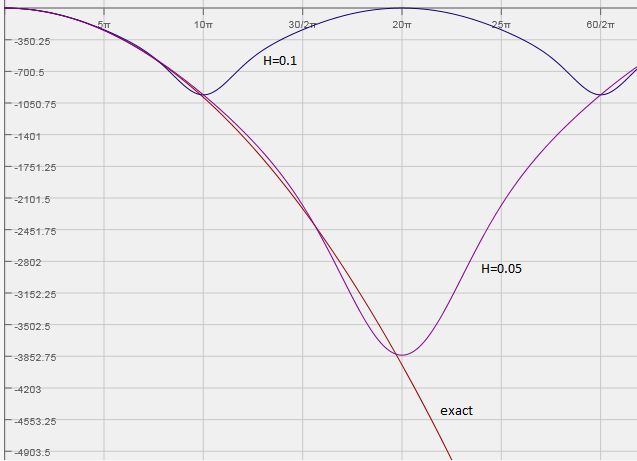
\includegraphics[width=0.8\textwidth]{figures/second-order-spectrum.png}
\caption{The exact spectrum ($\lambda$ versus $k$) of the linear diffusion equation, compared to a second-order approximation with $H=0.1$ and $H=0.05$, respectively, for $\gamma=1$.}
\label{fig:spec:2nd-order}
\end{figure}

%%%%%%%%%%%%%%%%%%%%%%%%%%%%%

\end{document}
